\documentclass{article}

\makeatletter
\renewcommand{\fnum@figure}{Εικόνα \thefigure}
\makeatother

\usepackage[greek, english]{babel}
\usepackage{alphabeta}
\usepackage{atbegshi, picture}

% Set page size and margins
% Replace `letterpaper' with`a4paper' for UK/EU standard size
\usepackage[letterpaper,top=2cm,bottom=2cm,left=3cm,right=3cm,marginparwidth=1.75cm]{geometry}
\newcommand\T{\rule{0pt}{2.6ex}}       % Top strut
\newcommand\B{\rule[-1.2ex]{0pt}{0pt}} 
% Useful packages
\usepackage{amsmath}
\usepackage{graphicx}
\usepackage[colorlinks=true, allcolors=blue]{hyperref}
\usepackage[utf8]{inputenc}
\usepackage{indentfirst}
\usepackage{hyperref} 
 \hypersetup{ 
     colorlinks=true, 
     linkcolor=blue, 
     filecolor=blue, 
     citecolor = black,       
     urlcolor=black, 
     } 

\addto\captionsenglish{
  \renewcommand{\contentsname}
    {Περιεχόμενα}
}

% \title{Feasibility Study}
% \date{}

\begin{document}
% \maketitle

\begin{titlepage}
   \begin{center}
       \vspace*{1cm}

       \textbf{\huge Project Plan}

       \vspace{0.5cm}
        Τεχνολογία Λογισμικού
            
       \vspace{1cm}

       \textbf{Μάριος Στεφανίδης\\Κούρου Αγγελική}
       
       
       \begin{figure}[!htb]
        \centering
        
\includegraphics[width=0.5\textwidth]{logo.png}
        \end{figure}
        
        \vspace{0.5cm}
        
        \begin{figure}[!htb]
        \centering
        \includegraphics[width=0.5\textwidth]{UoP.jpg}
        \end{figure}


       \vfill
            
       Τεχνικό Κείμενο για την Τεχνολογία Λογισμικού\\
            
       \vspace{0.5cm}
            
       CEID, ECE\\
       University of Patras\\
            
   \end{center}
\end{titlepage}



\noindent Η ομάδα μας

\begin{enumerate}
  \item Βεργίνης Δημήτριος, ΑΜ: 1066634 , ECE
  \item Βλαχογιάννης Δημήτριος, ΑΜ: 1067371, CEID
  \item Κούρου Αγγελική, ΑΜ: 1067499 , CEID
  \item Μητροπούλου Αικατερίνα - Quality Manager, ΑΜ: 1067409, CEID
  \item Στεφανίδης Μάριος - Project Manager, ΑΜ:1067458, CEID
\end{enumerate}

\section{Εισαγωγή}

Παρακάτω παρουσιάζονται τα διαγράμματα ευρωστίας των σεναρίων χρήσης του \textbf{Medic World}. \vspace{0.2cm}

\underline{Σημείωση:} Κάθε μέλος της ομάδας ανέλαβε από δύο διαγράμματα ευρωστίας (robustness \par diagrams) αλλά την οργάνωση και τη σύνταξη της αναφοράς ανέλαβαν οι Κούρου Αγγελική και \par Στεφανίδης Μάριος.  


\section{Ενέργειες στην Καρτέλα Ασθενούς}

\vspace{0.2cm}

\begin{figure}[!htb]
        \centering
        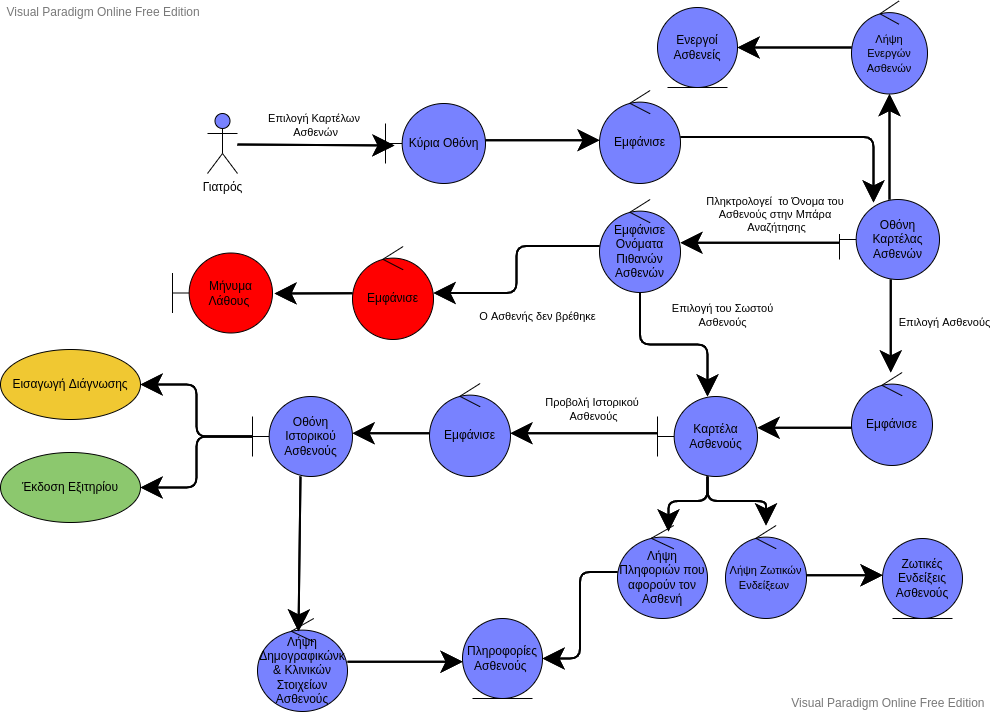
\includegraphics[width=1\textwidth]{Patient Card.png}
\end{figure}

\newpage

\subsubsection{Εισαγωγή Διάγνωσης}

\vspace{0.2cm}

\begin{figure}[!htb]
        \centering
        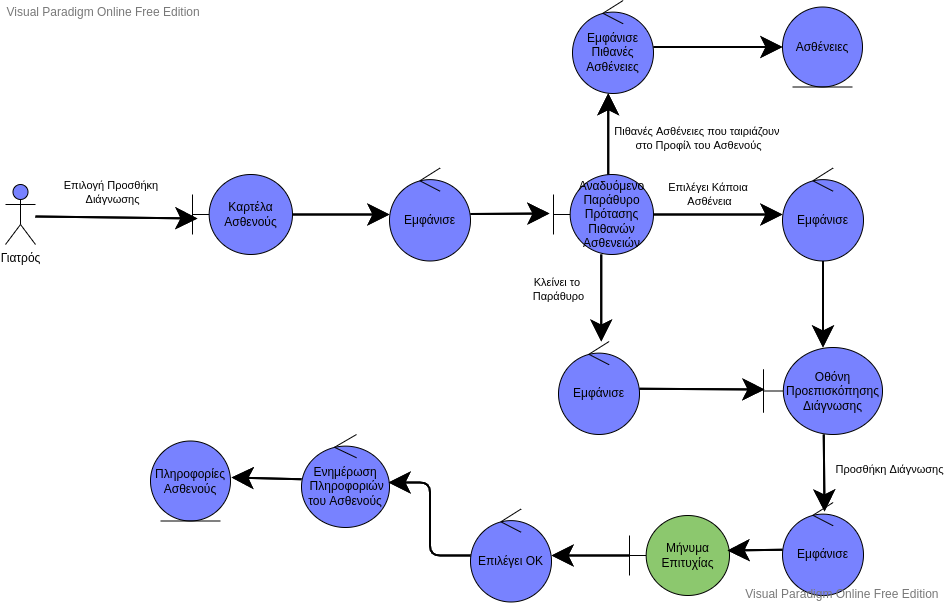
\includegraphics[width=1.1\textwidth]{Patient Card - Diagnosis.png}
\end{figure}

\newpage

\subsubsection{Έκδοση Εξιτηρίου}

\vspace{0.2cm}

\begin{figure}[!htb]
        \centering
        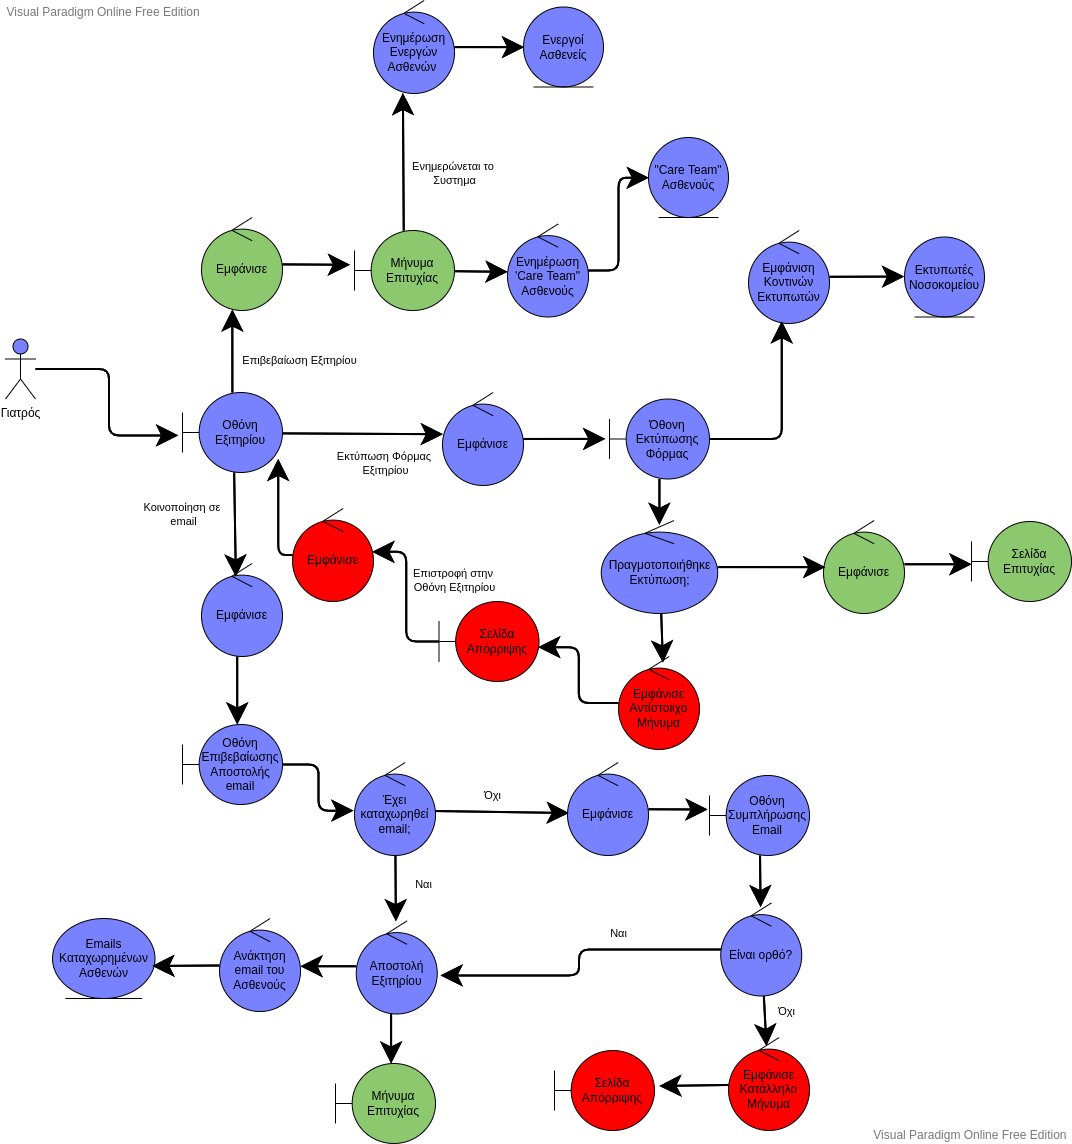
\includegraphics[width=1.1\textwidth]{Patient Card - Discharge.png}
\end{figure}

\newpage

\section{Απασχόληση Χειρουργείου}

\vspace{0.2cm}

\begin{figure}[!htb]
        \centering
        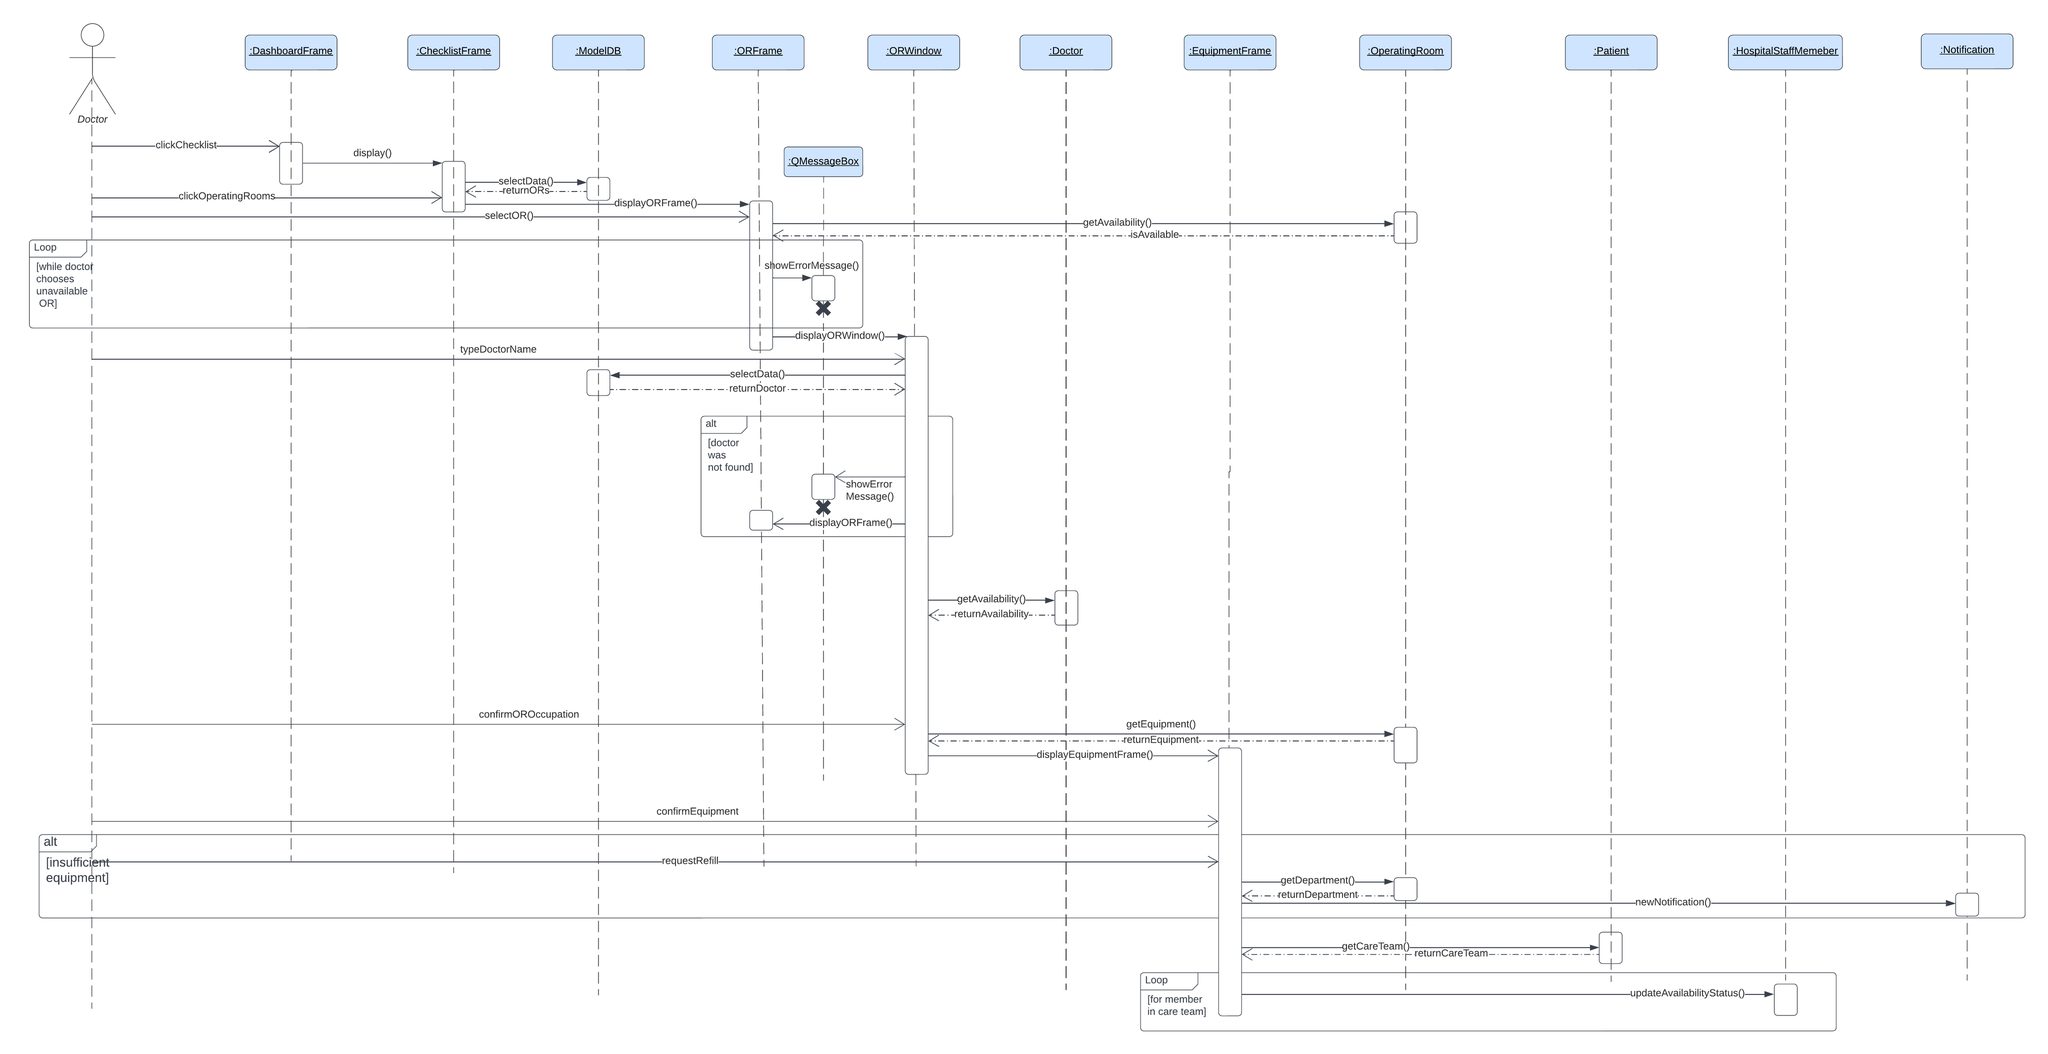
\includegraphics[width=1.1\textwidth]{OR Occupation.png}
\end{figure}

\newpage

\section{Αποστολή Μηνύματος}

\vspace{0.2cm}

\begin{figure}[!htb]
        \centering
        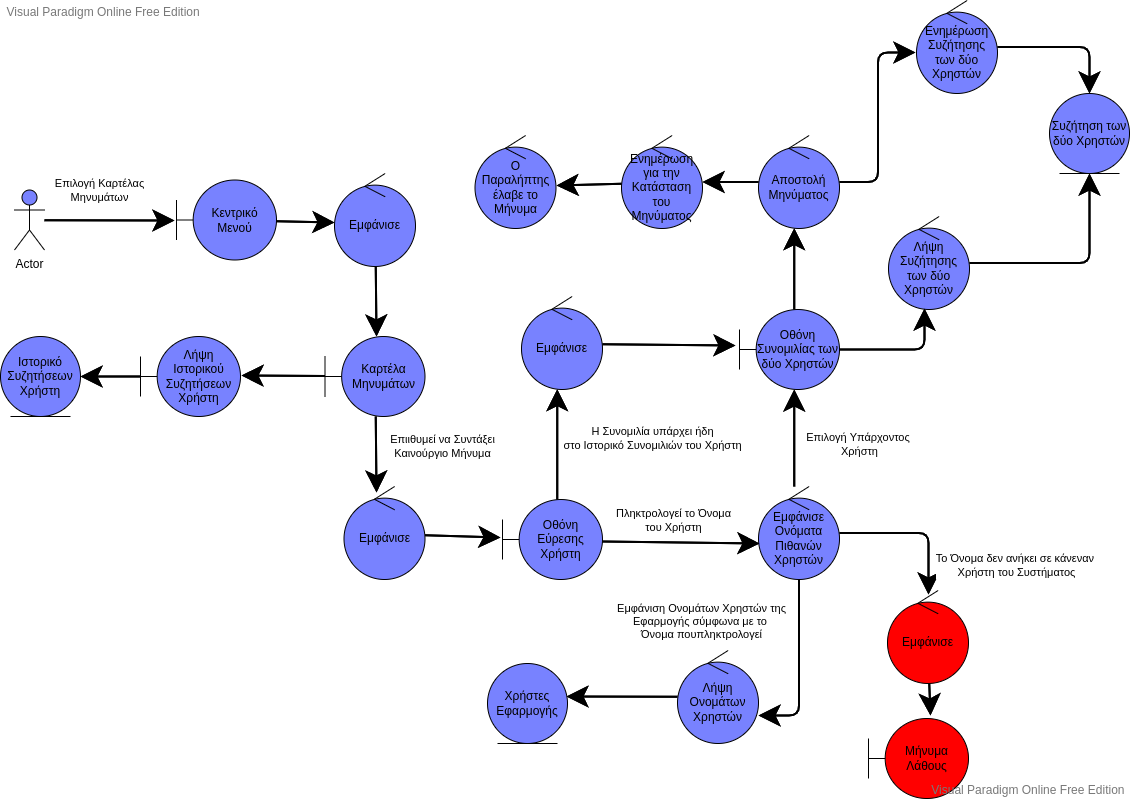
\includegraphics[width=1\textwidth]{Messages.png}
\end{figure}

\newpage

\section{Έγκριση και Διεξαγωγή Εξετάσεων}

\vspace{0.2cm}

\begin{figure}[!htb]
        \centering
        \includegraphics[width=1\textwidth]{Εxaminations Conduction.png}
\end{figure}

\newpage

\section{Έγκριση Δημοσίευσης}

\vspace{0.2cm}

\begin{figure}[!htb]
        \centering
        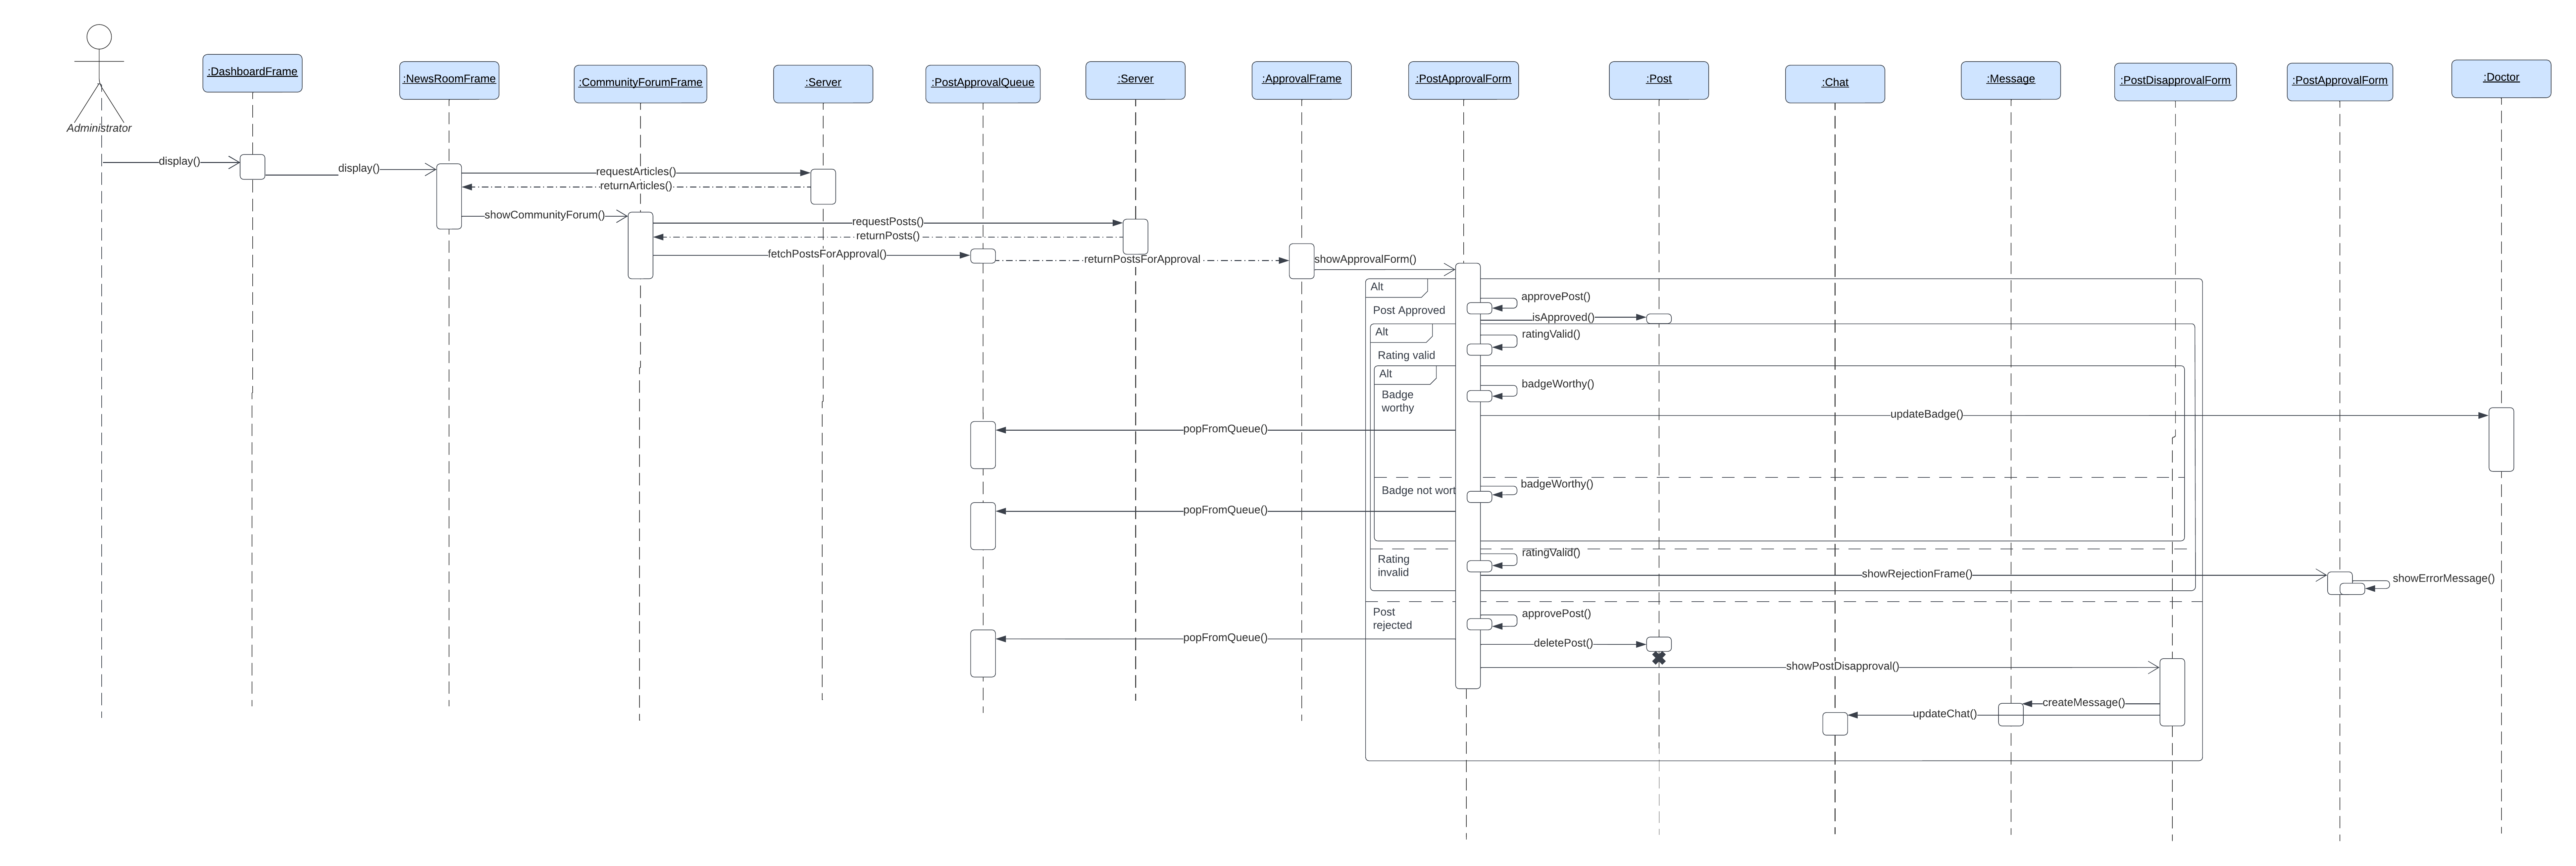
\includegraphics[width=1\textwidth]{Admin Approval.png}
\end{figure}

\newpage

\section{Δημιουργία Δημοσίευσης}

\vspace{0.2cm}

\begin{figure}[!htb]
        \centering
        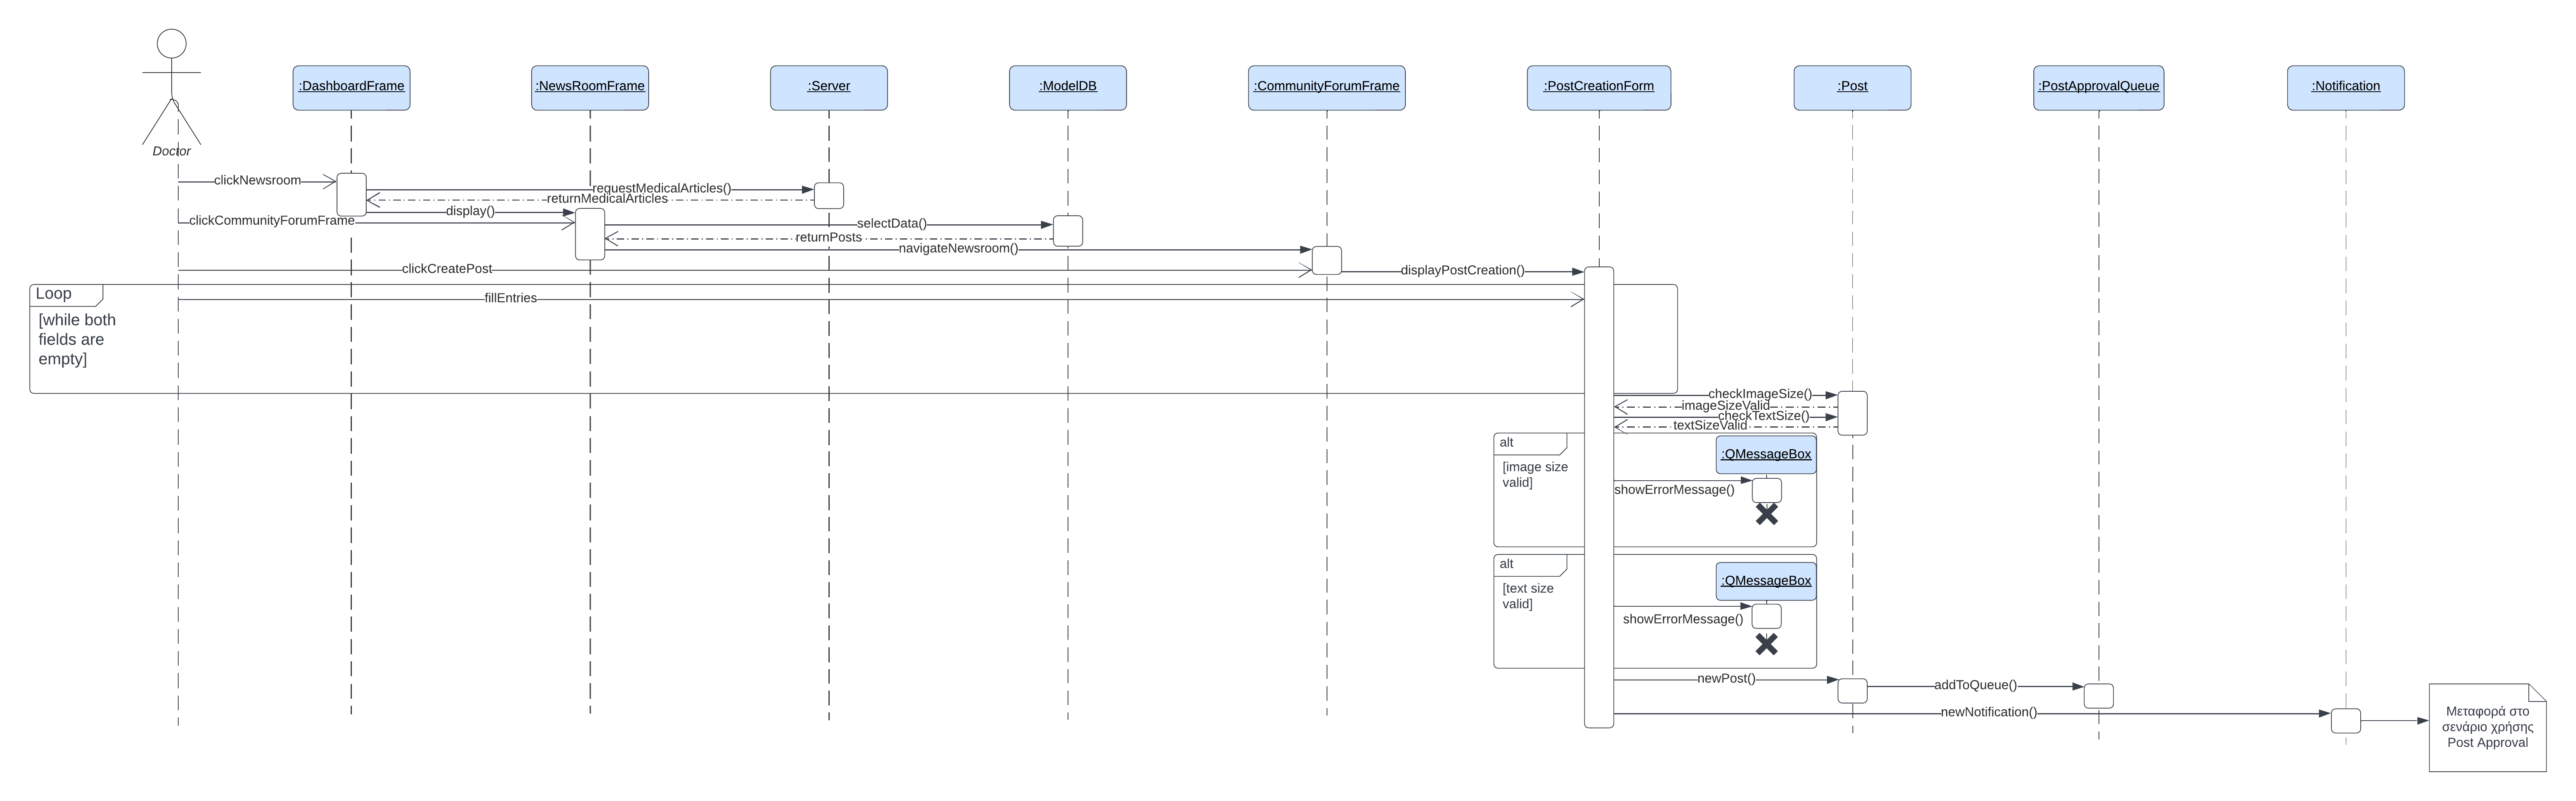
\includegraphics[width=1\textwidth]{Create Post.png}
\end{figure}

\newpage

\section{Δημιουργία Εκδήλωσης}

\vspace{0.2cm}

\begin{figure}[!htb]
        \centering
        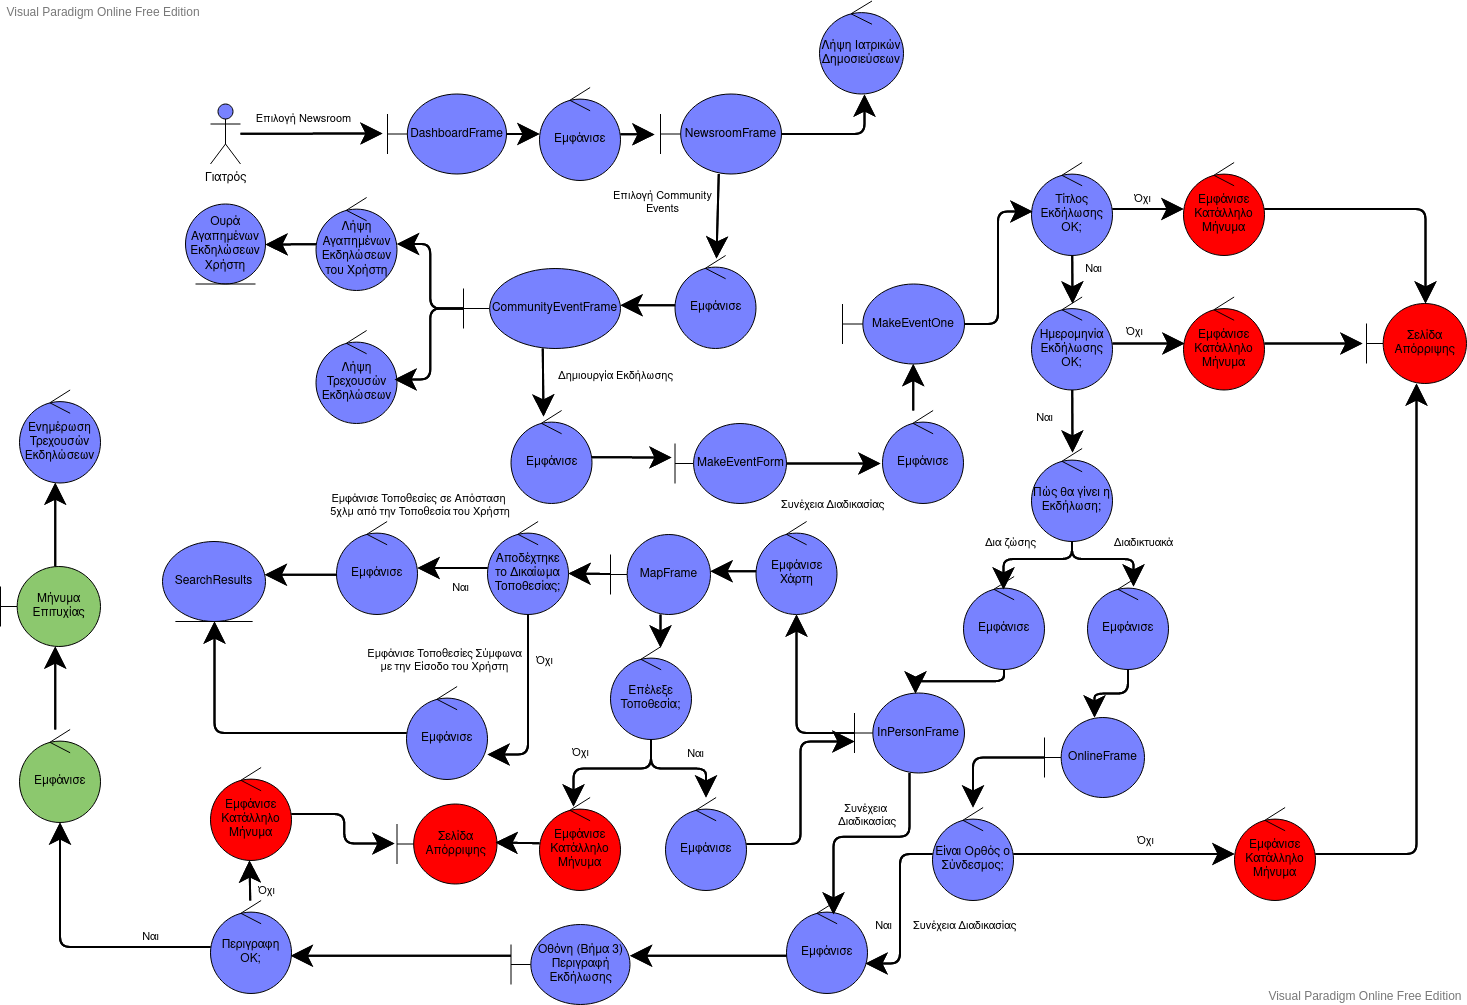
\includegraphics[width=1.1\textwidth]{Make Event.png}
\end{figure}

\newpage

\section{Καταχώρηση/Εισαγωγή Ασθενούς}

\vspace{0.2cm}

\begin{figure}[!htb]
        \centering
        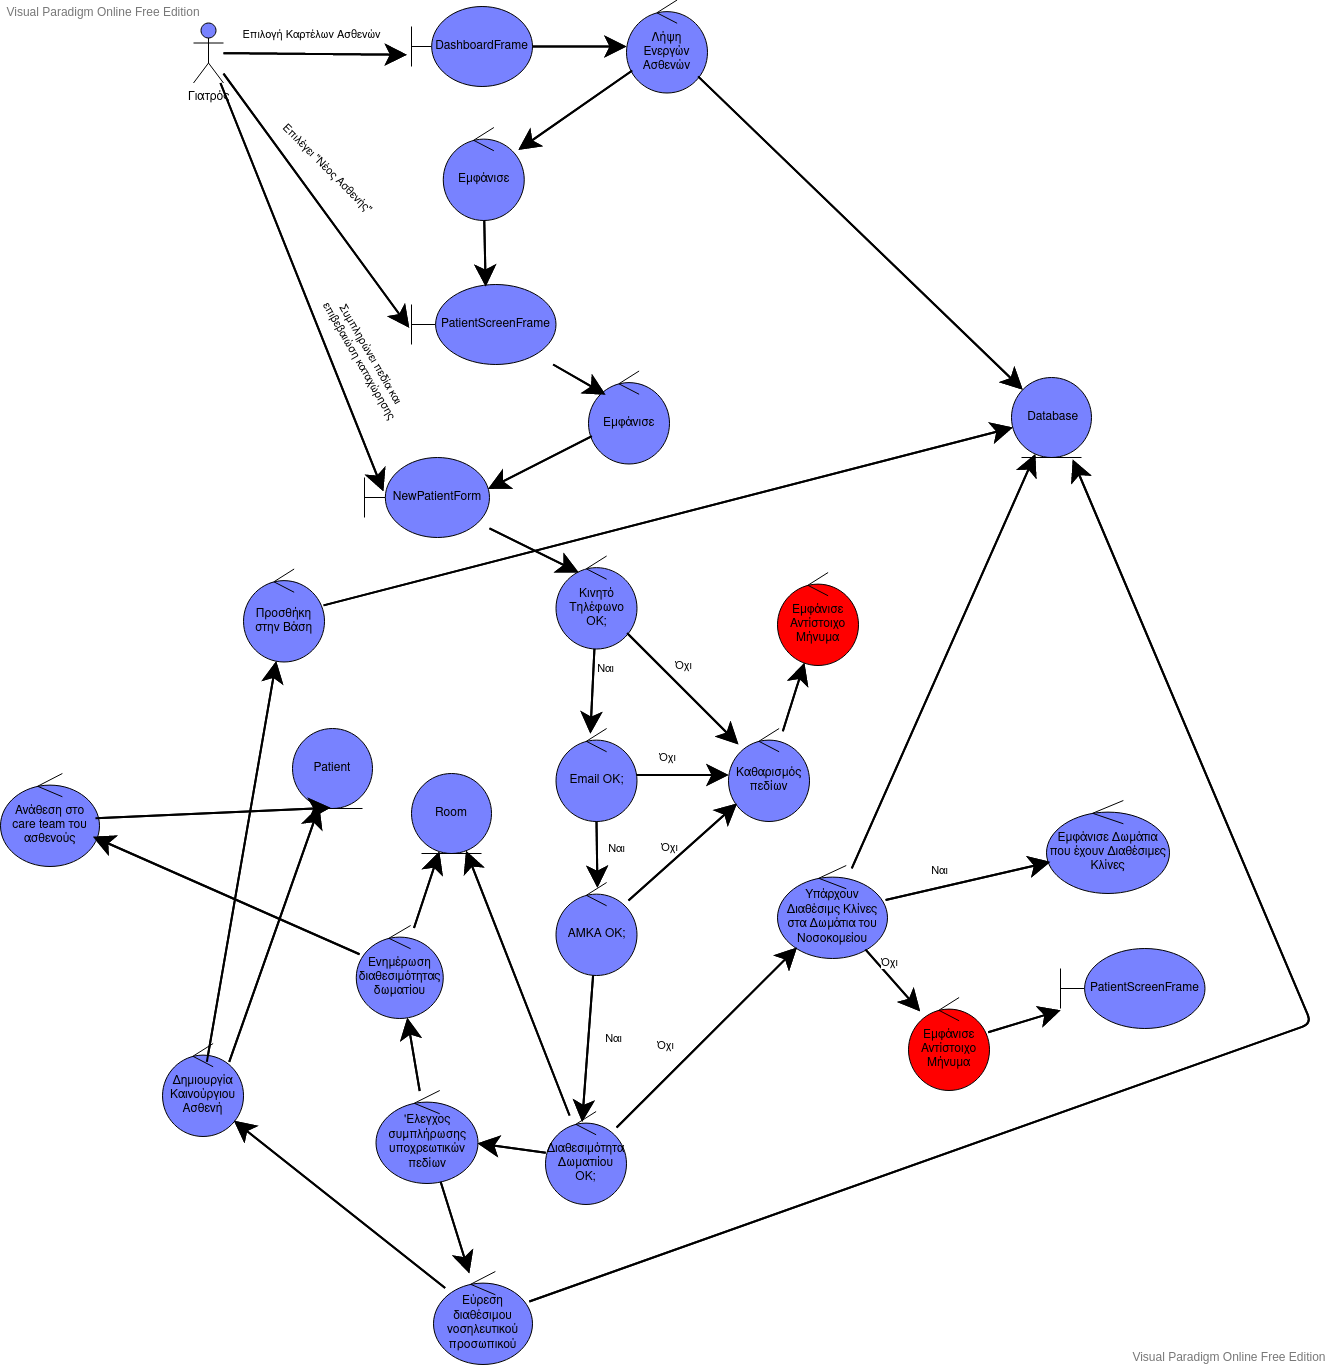
\includegraphics[width=1\textwidth]{Patient Insertion.png}
\end{figure}

\newpage

\section{Καταχώρηση Νέου Μέλους του Προσωπικού}

\vspace{0.2cm}

\begin{figure}[!htb]
        \centering
        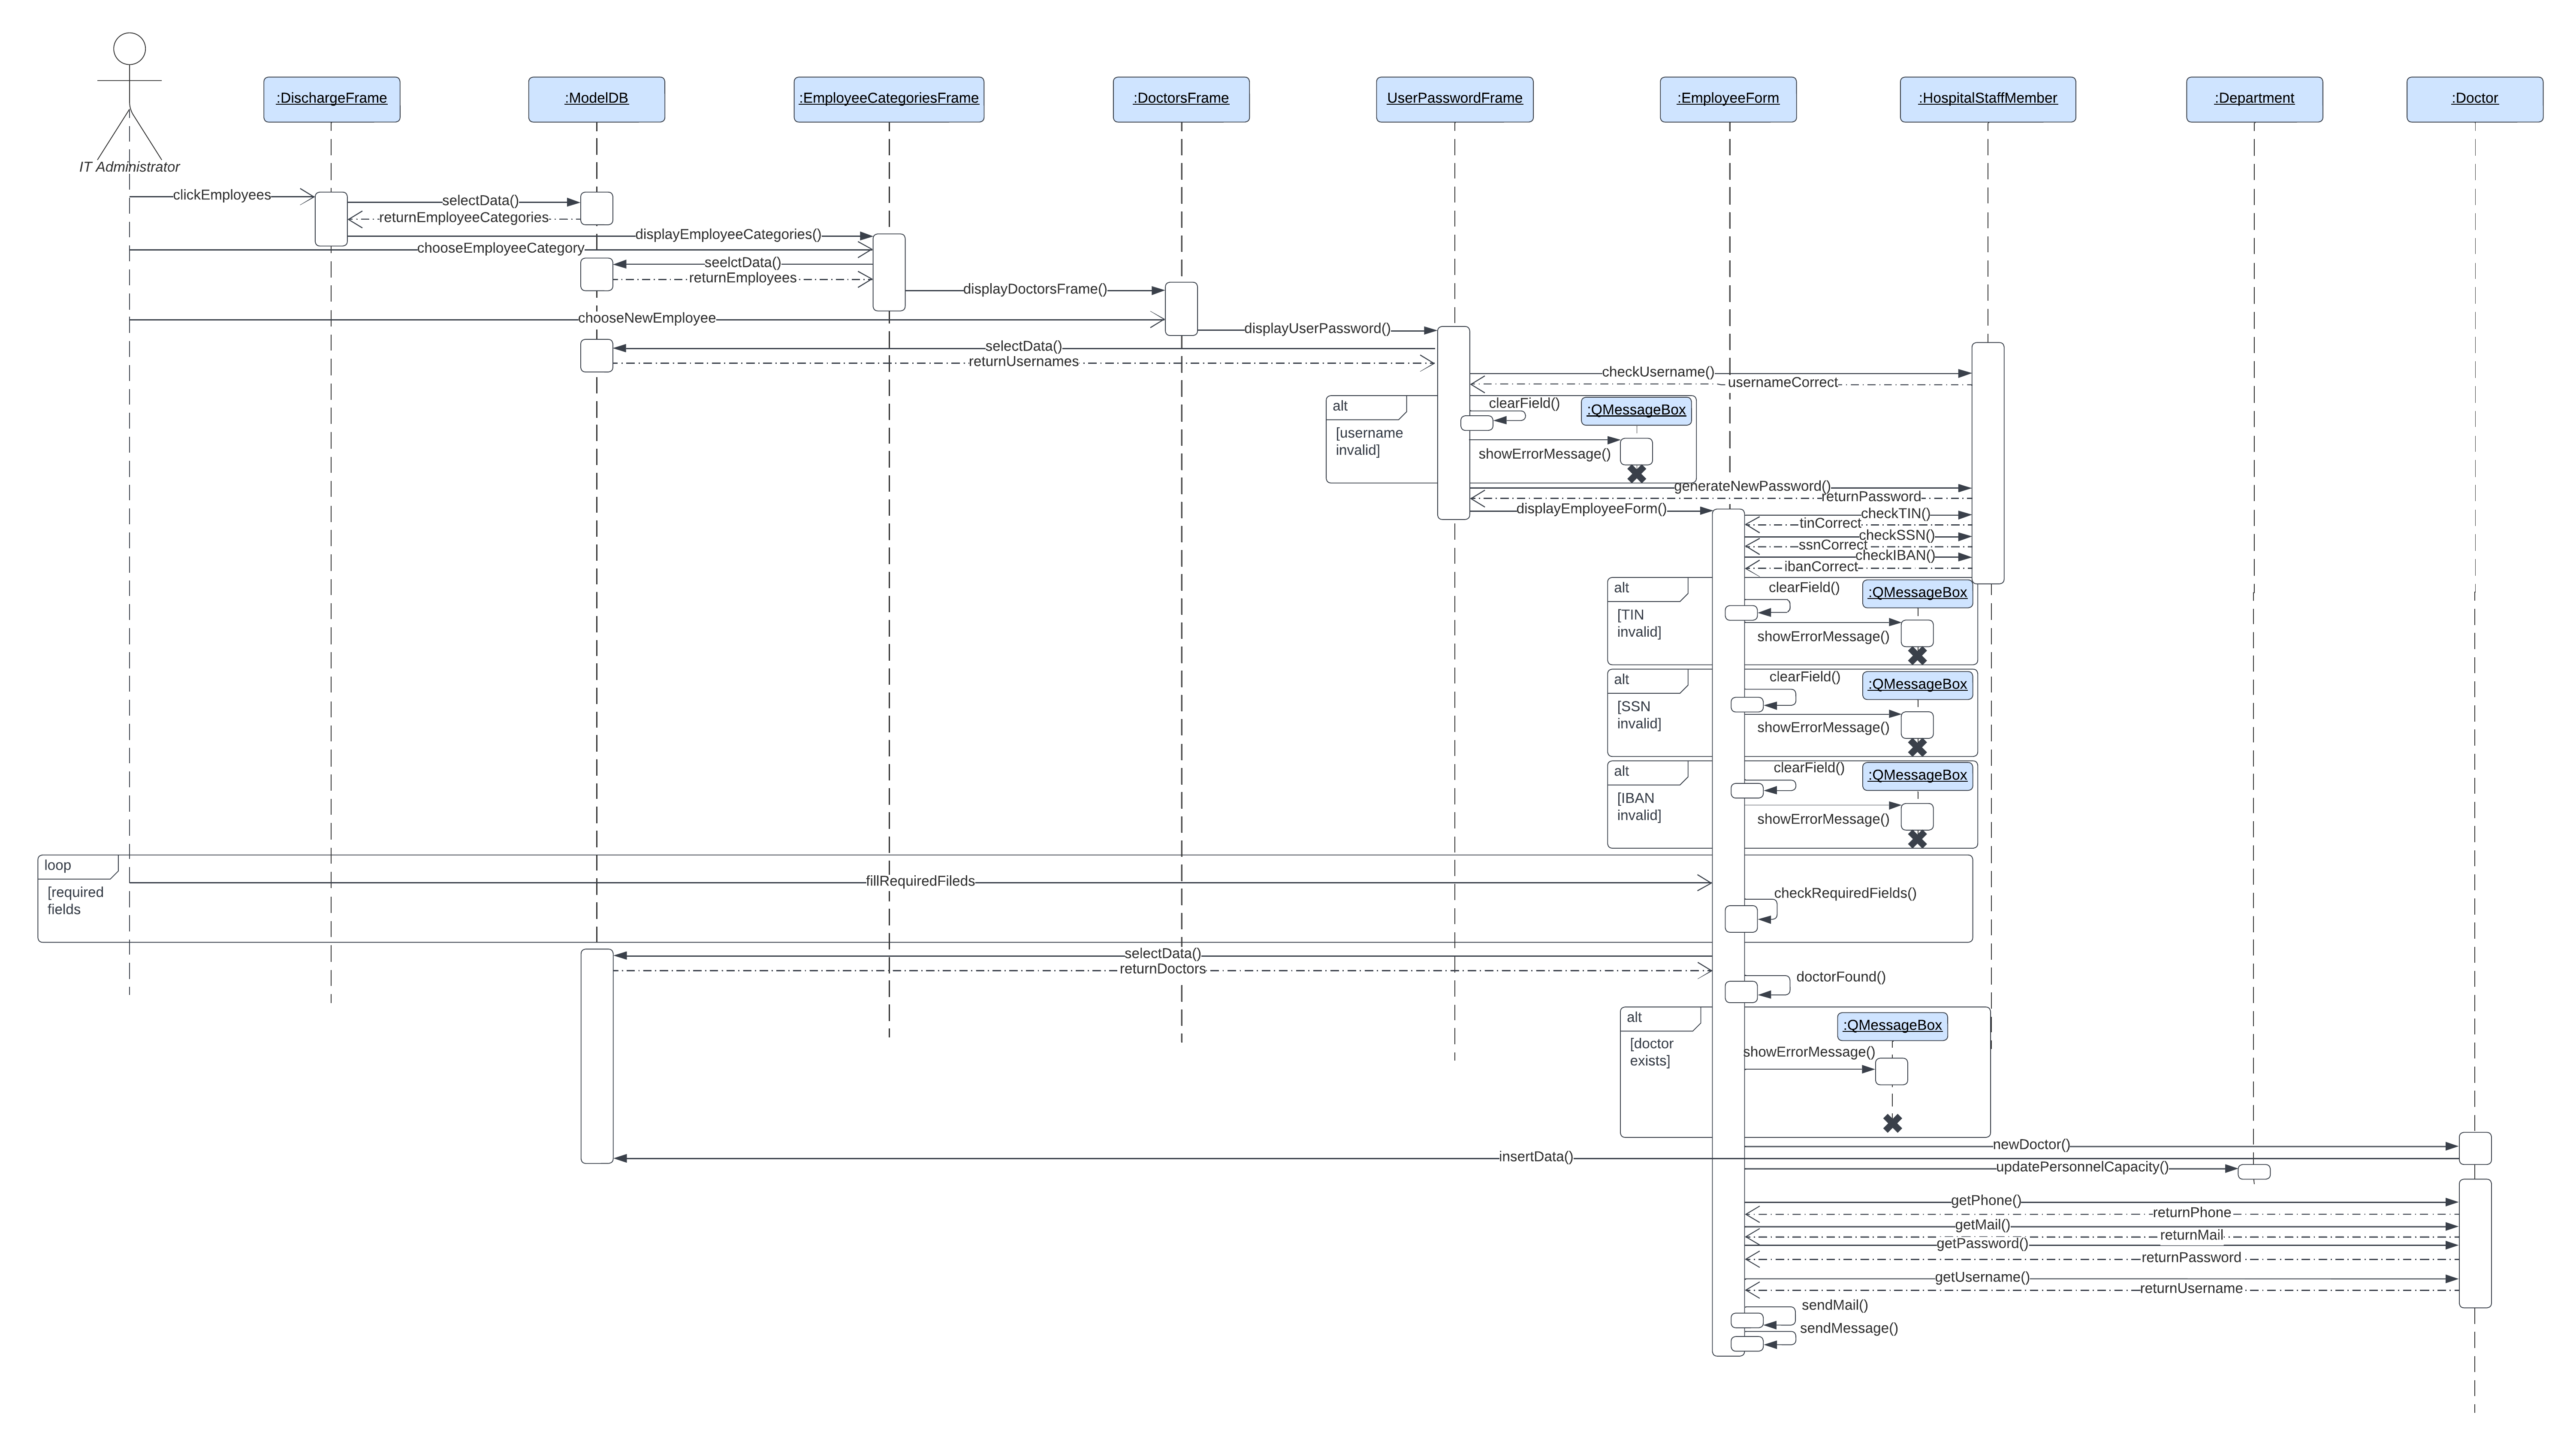
\includegraphics[width=1\textwidth]{Employee Insertion.png}
\end{figure}

\newpage

\section{Καταχώρηση Νέου Φαρμάκου}

\vspace{0.2cm}

\begin{figure}[!htb]
        \centering
        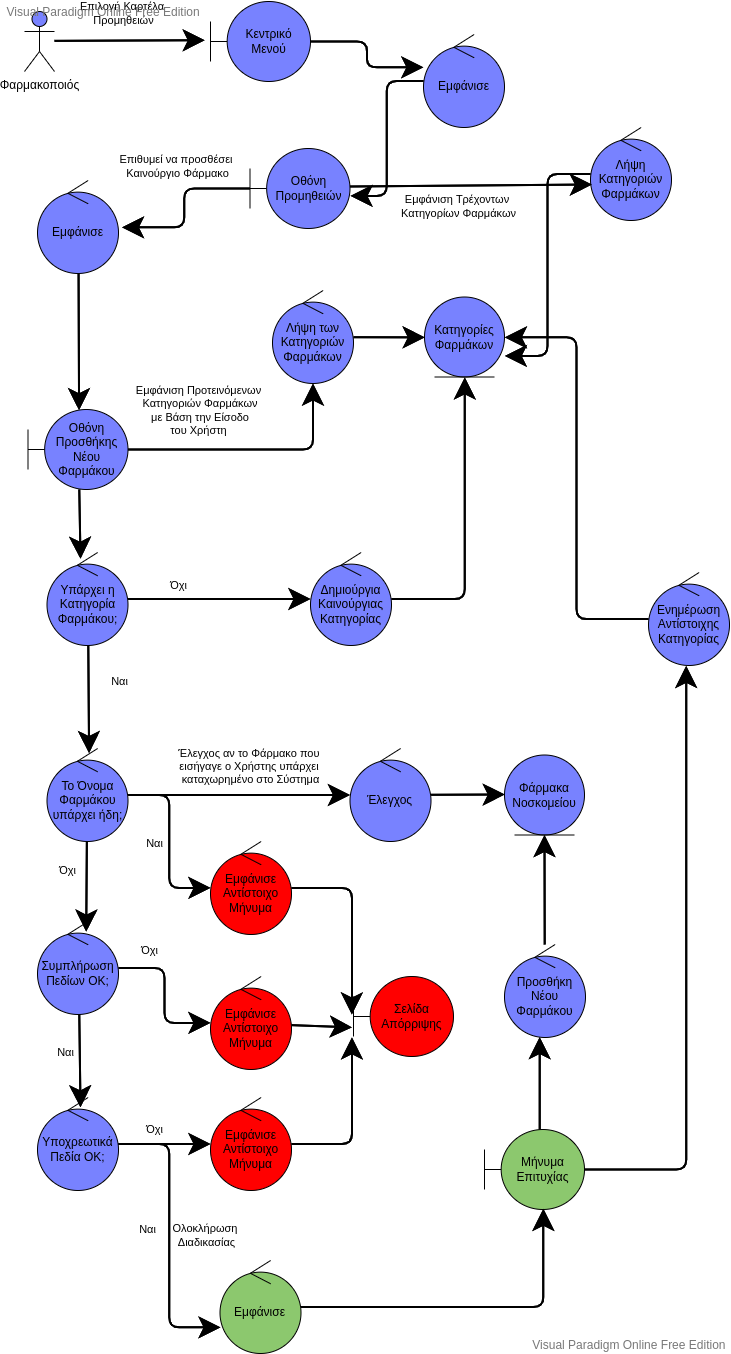
\includegraphics[width=0.7\textwidth]{Medicine Insertion.png}
\end{figure}



\end{document}
